グラフ演算時にはメモリへの不規則なアクセスによるキャッシュミスが多発する.\cite{wei2016speedup} では,sd1-arc データセット (9,500万ノード,19 億エッジ)
を使用し,代表的なグラフアルゴリズムである 
Breadth-First Search (BFS) \cite{cormen2009introduction},Depth-First Search (DFS) \cite{cormen2009introduction},
Strongly Connected Component (SCC) \cite{sharir1981strong},Shortest Path (SP) \cite{cormen2009introduction},
PageRank (PR),Dominating Set (DS) \cite{cockayne1978domination},Graph Decomposition (Kcore) \cite{batagelj2003m},Graph Diameter (Diam) を
実行したところ, 演算時間全体の内,キャッシュミスに伴うメインメモリへのアクセス時間が占める平均割合は約 70 \% であると報告されている.
図 \ref{cache_miss_ratio}に示されているように,演算時間全体に対し,キャッシュミスに伴うメインメモリへのアクセス時間が占める割合は極めて高い.
つまり,演算時のキャッシュミスを減少させることで,演算時間を減少させることが可能である.
\begin{figure}[t]
  \centering
  %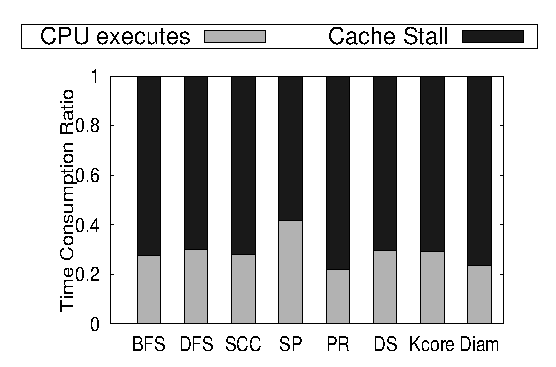
\includegraphics[width=\linewidth]{./figure/cache_miss.pdf}
  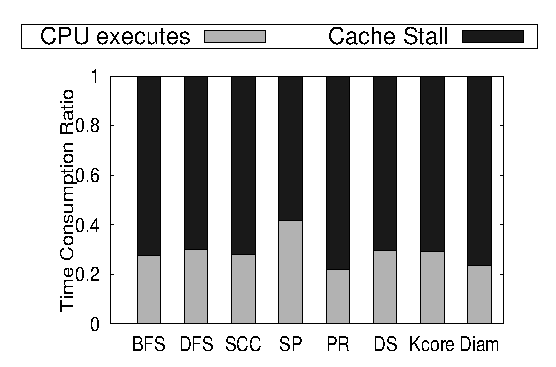
\includegraphics[scale=1.0]{./figure/cache_miss.pdf}
  \caption{演算時間全体に対しキャッシュミスに伴うメインメモリへのアクセス時間が占める割合}
  \label{cache_miss_ratio}
\end{figure}

ノード ID の再配置では,グラフ演算に伴うメモリアクセスの特徴を考慮することで,キャッシュミス減少を実現する.
また,ノード ID の配置を変更するだけなので,グラフアルゴリズムやデータ構造自体を変更する必要はなく,既存のグラフ処理系に対して容易に適用することが可能である.

グラフ演算では各ノードが PR での重要度や BFS での始点からの距離などといった,アルゴリズム固有の値を保持している.
一般に,これらの値は図 \ref{id_index}で示すように,ノード ID をインデックスとする配列に格納される.
\begin{figure}[t]
  \centering
  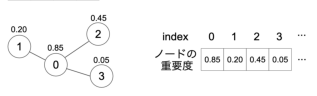
\includegraphics[width=\linewidth]{./figure/id_index.pdf}
  \caption{ノード ID をインデックスとする配列での格納}
  \label{id_index}
\end{figure}
そのため,ID が連続するノードの値はメモリ上で連続して格納され,ID が近いノードの値は同一キャッシュブロックに属する.
図\ref{cache_block}で示すように,ノード ID X の値が参照され,キャッシングがされる場合,X 前後の ID を持つノードもまとめてキャッシングされる.
\begin{figure}[t]
  \centering
  %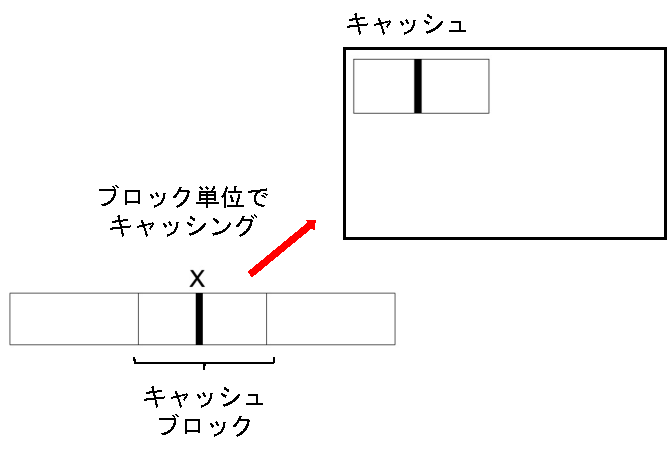
\includegraphics[width=\linewidth]{./figure/cache_block.pdf}
  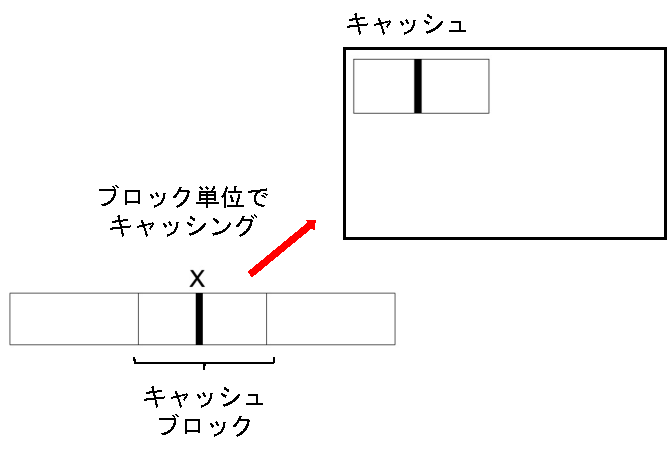
\includegraphics[scale=1.0]{./figure/cache_block.pdf}
  \caption{ブロック単位でのキャッシング}
  \label{cache_block}
\end{figure}
グラフ演算では演算過程において隣接ノードの値を参照とするという操作が繰り返されるため,ノード ID の配置方法によりキャッシュの使用効率も変化する.
そこで,グラフを取得しながらノード ID を再配置するにあたり,特に ID の連続性と演算時のアクセス局所性が重要となる.
\section{ID の連続性}
既存手法では,グラフの全体構造を把握した上で再配置を行うので,全ノードに連続した ID が再配置されることが保証される.
しかし,グラフを取得しながら ID を再配置する場合,再配置する ID が連続的かどうかを考慮する必要がある.
ID が連続するノードの値はメモリ上でも連続して格納されるが,ID の連続性が欠如していると,各ノードの値がメモリ上で点在する形となり,
全ノードを格納するためのキャッシュブロック数が増加してしまう.
キャッシュブロック数の増加に伴い,演算時にアクセス対象となるブロック数も増加し,
キャッシュブロックの書き換えが頻発してしまうためキャッシュミスが増加する.
例えば,図\ref{id_not_consecutive} で示すように,ノード ID が 2, 6, 10, 37, 53 と非連続的で,これら 5 ノードの値を格納するために
必要なブロック数が 3 だとする.
このグラフのノード ID を図\ref{id_consecutive} で示すように再配置する.
ID の連続性を実現した再配置により,同一の 5 ノードを格納するために必要なブロック数が 1 に減少している.
\begin{figure}[t]
  \begin{tabular}{cc}
    \begin{minipage}[t]{0.45\hsize}
      \centering
      %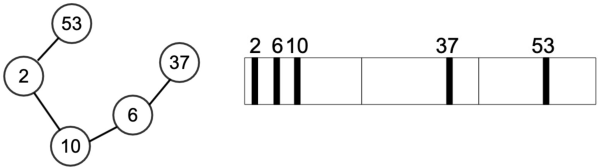
\includegraphics[keepaspectratio, scale=0.50]{./figure/id_not_consecutive.pdf}
      %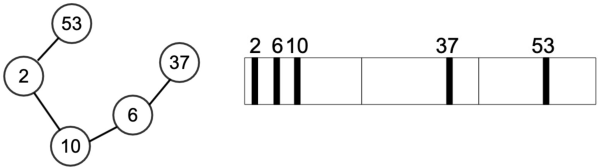
\includegraphics[keepaspectratio, width=7cm]{./figure/id_not_consecutive.pdf}
      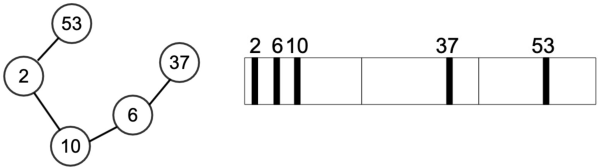
\includegraphics[width=7cm]{./figure/id_not_consecutive.pdf}
      %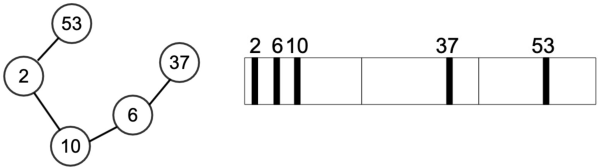
\includegraphics[scale=0.50]{./figure/id_not_consecutive.pdf}
      \caption{ID が非連続的な場合のブロック数}
      \label{id_not_consecutive}
    \end{minipage} &
    \begin{minipage}[t]{0.45\hsize}
      \centering
      %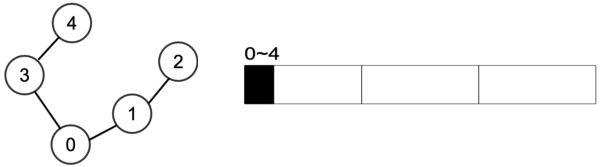
\includegraphics[keepaspectratio, scale=0.50]{./figure/id_consecutive.pdf}
      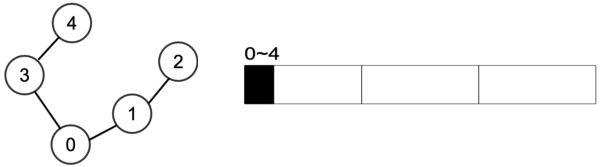
\includegraphics[width=7cm]{./figure/id_consecutive.pdf}
      %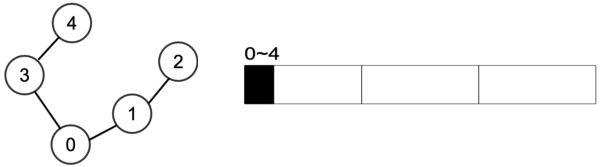
\includegraphics[scale=0.50]{./figure/id_consecutive.pdf}
      \caption{ID が連続的な場合のブロック数}
      \label{id_consecutive}
    \end{minipage}
  \end{tabular}
\end{figure}
\section{演算時のアクセス局所性}
グラフを取得しながら ID を再配置する場合でも,既存手法と同様に演算時のアクセス局所性を考慮する必要がある.
具体的には,演算時に局所的なアクセスが発生するノード群を同一キャッシュブロックに格納しておくことで,
キャッシュの使用効率が向上し,キャッシュミスが減少する.
アクセス局所性は次数による局所性と近接構造による局所性に分類できる.
\subsection{次数による局所性}
実世界グラフは次数分布が冪乗則に従うスケールフリー性と呼ばれる性質を持つ\cite{barabasi1999emergence,faloutsos1999power,clauset2009power}.
スケールフリー性を持つグラフでは,極めて少数のノードが高い次数を持つ一方で,大多数のノードは低い次数を持つ.
グラフ演算における各ノードへのアクセス頻度はそのノードの次数に比例するため,
少数の高次数ノードへアクセスが集中する.
このように,グラフがスケールフリー性を持つ状況では,次数が同程度のノードが同一キャッシュブロックに格納されるように ID を再配置することが有効である.

図\ref{bad_degree_cache} で示すように,同一キャッシュブロック内に次数が大きく異なるノードの値が格納されている場合,
低次数ノードの値は高次数ノードへのアクセスに伴って頻繁にキャッシングされる.
グラフ演算において低次数ノードへのアクセス数は極めて小さいため,
アクセスされにくい値の頻繁なキャッシングはキャッシュの使用効率低下を引き起こす.
一方,図\ref{good_degree_cache} で示すように,同一キャッシュブロック内に同程度の次数を持つノードの値が格納されている場合,
高次数ノードのアクセスに伴い低次数ノードの値がキャッシングされることを防止できる.
これにより,高次数ノードの値を格納しているブロックは演算終了時までキャッシュに格納され続け,
低次数ノードの値を格納しているブロックは必要最低限の回数だけキャッシングされるため,演算時のキャッシュミスが減少する.


\begin{figure}[t]
  \begin{tabular}{cc}
    \begin{minipage}[t]{0.45\hsize}
      \centering
      %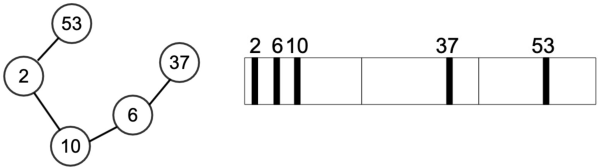
\includegraphics[keepaspectratio, scale=0.50]{./figure/id_not_consecutive.pdf}
      %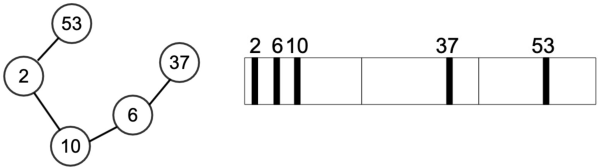
\includegraphics[keepaspectratio, width=7cm]{./figure/id_not_consecutive.pdf}
      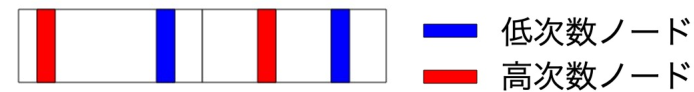
\includegraphics[width=7cm]{./figure/bad_degree_cache.pdf}
      %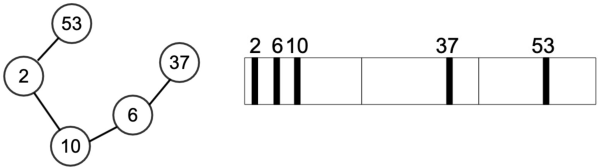
\includegraphics[scale=0.50]{./figure/id_not_consecutive.pdf}
      \caption{ブロック内のノードの次数に差がある場合}
      \label{bad_degree_cache}
    \end{minipage} &
    \begin{minipage}[t]{0.45\hsize}
      \centering
      %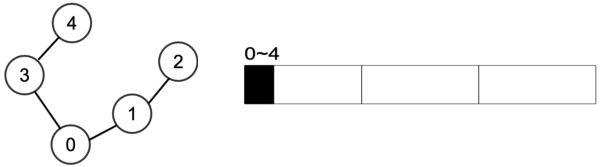
\includegraphics[keepaspectratio, scale=0.50]{./figure/id_consecutive.pdf}
      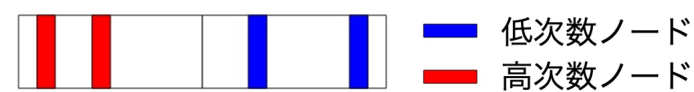
\includegraphics[width=7cm]{./figure/good_degree_cache.pdf}
      %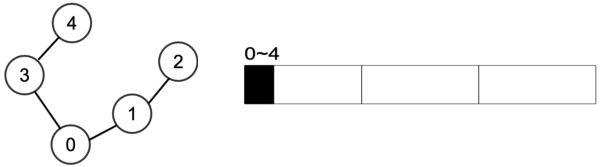
\includegraphics[scale=0.50]{./figure/id_consecutive.pdf}
      \caption{ブロック内のノードの次数が同程度の場合}
      \label{good_degree_cache}
    \end{minipage}
  \end{tabular}
\end{figure}

%なお,次数による局所性に着目した ID 再配置手法として \cite{zhang2017making,faldu2019closer}が提案されている.
\subsection{近接構造による局所性}
実世界グラフはスケールフリー性だけでなく,コミュニティ構造を保有するという特徴を持つ\cite{girvan2002community,leskovec2009community}.
コミュニティとは,グラフ上で密に接続しあっているノードの集合であり,同一コミュニティに所属するノードはグラフ上で極めて近接している.
%コミュニティ内のノード群は密に接続しあっており,グラフ上で極めて近接している.
一般に,グラフ演算では隣接ノードの値を参照するという操作が繰り返されるため,コミュニティ内のノード間で局所的なアクセスが発生する.
そのため,同一コミュニティに属する極めて近接したノード群の値が同一キャッシュブロックに格納されるように ID を再配置することが有効である.

例えば,図\ref{bad_community_cache}で示すように,ID V のノードに対し,その隣接ノードの ID が 2, 37, 53 と離れている場合,
ノード V の隣接ノードの値を参照するためには,3つのキャッシュブロックにアクセスする必要があるとする.
この場合,図\ref{good_community_cache}で示すように,隣接ノードが近い ID を持つように ID を再配置することで,
全隣接ノードが同一キャッシュブロックに格納され,演算時には1つのキャッシュブロックへアクセスするだけでノード V の全隣接ノードの値を参照することが可能となる.
このように,グラフ上で近接しているノードが同一キャッシュブロックへ格納されるように ID を再配置することで,演算全体を通してアクセスする
ブロック数が減少し,キャッシュミスが減少する.
\begin{figure}[t]
  \begin{tabular}{cc}
    \begin{minipage}[t]{0.45\hsize}
      \centering
      %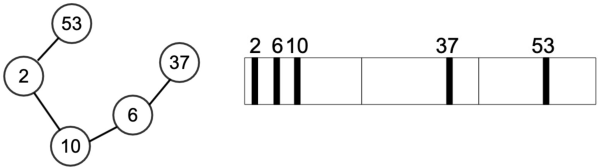
\includegraphics[keepaspectratio, scale=0.50]{./figure/id_not_consecutive.pdf}
      %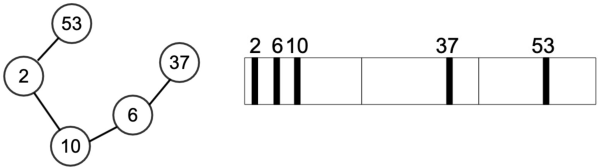
\includegraphics[keepaspectratio, width=7cm]{./figure/id_not_consecutive.pdf}
      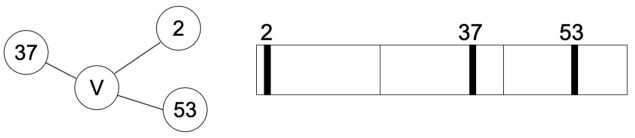
\includegraphics[width=7cm]{./figure/bad_community_cache.pdf}
      %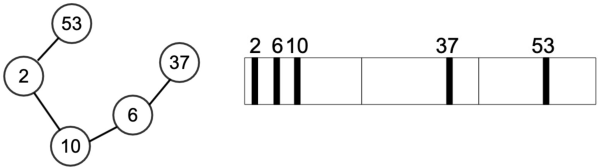
\includegraphics[scale=0.50]{./figure/id_not_consecutive.pdf}
      \caption{近接ノードの ID が離れている場合}
      \label{bad_community_cache}
    \end{minipage} &
    \begin{minipage}[t]{0.45\hsize}
      \centering
      %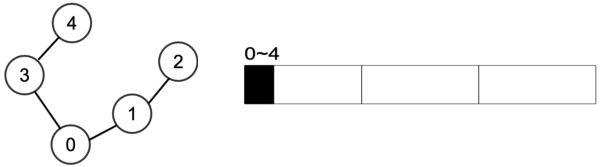
\includegraphics[keepaspectratio, scale=0.50]{./figure/id_consecutive.pdf}
      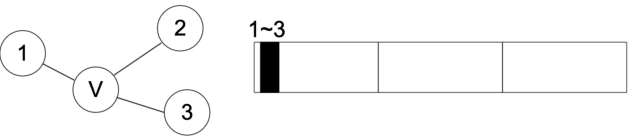
\includegraphics[width=7cm]{./figure/good_community_cache.pdf}
      %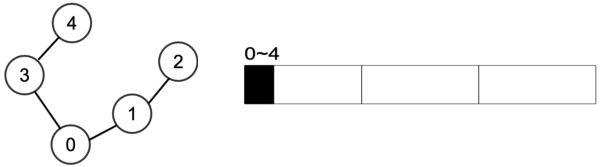
\includegraphics[scale=0.50]{./figure/id_consecutive.pdf}
      \caption{近接ノードの ID が近い場合}
      \label{good_community_cache}
    \end{minipage}
  \end{tabular}
\end{figure}

\section{自律分散グラフ管理環境での課題}
既存手法はグラフの全体構造を把握している前提で議論がされているため,再配置の対象となるノード数は既知である.
予めノード数が判明していることで ID の連続性が保証されているが,グラフ取得が完了するまで全グラフが手元にない状況では
既存手法と同様に ID の連続性を保証することは不可能である.
グラフ取得をしながら ID の連続性を保った再配置を実行するには,取得途中のグラフに対して連続的な ID を再配置し続ける必要がある.
しかし,取得途中のグラフ構造には次数による局所性や近接構造による局所性などの特徴が十分に反映されない可能性が高い.
例えば,取得初期の段階で高次数ノードと判定されたノードが取得完了時点では低次数ノードであると判明する可能性がある点や,
取得途中ではグラフ上の近接構造を正確に把握することが困難な点などが挙げられる.
ID の連続性のみを意識して再配置を行うと演算時のアクセス局所性が損なわれてしまうが,
アクセス局所性のみを意識するとグラフの取得完了を待つコストが増加してしまう.
このように,グラフ取得が完了するまで全グラフが手元にない状況では連続性とアクセス局所性の完全な両立は困難である.